\documentclass[tikz]{standalone}
\usepackage{pgfplots}
\pgfplotsset{compat=1.15}
\usepackage{mathrsfs}
\usetikzlibrary{arrows,calc}
\usepackage{tkz-euclide}

\pagestyle{empty}

\definecolor{AngleClr}{rgb}{0,0.39215686274509803,0}
\definecolor{ShapeClr}{rgb}{0.6,0.2,0}

\begin{document}

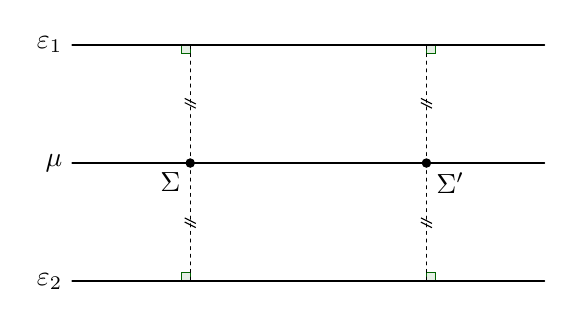
\begin{tikzpicture}[scale=.75]
\tkzSetUpLine[line width=1pt,color=black]
\tkzSetUpPoint[fill=black]

\tkzDefPoints{0/0/A,8/0/B,0/-4/C,8/-4/D,0/-2/E,8/-2/F,2/-2/S,6/-2/SS}
\tkzDefPoints{2/0/S1,2/-4/S2,6/0/SS1,6/-4/SS2}

\tkzMarkRightAngles[line width=0.5pt, size=.15,color=AngleClr,fill=AngleClr,fill opacity=0.1](S,S1,A S,S2,C)

\tkzMarkRightAngles[line width=0.5pt, size=.15,color=AngleClr,fill=AngleClr,fill opacity=0.1](SS,SS1,B SS,SS2,D)

\tkzDrawSegments[line width=0.5pt,color=black](A,B C,D E,F)

\tkzDrawSegments[line width=0.5pt,color=black,dashed,dash pattern=on 1pt off 1.75pt](S,S1 S,S2)

\tkzDrawSegments[line width=0.5pt,color=black,dashed,dash pattern=on 1pt off 1.75pt](SS,SS1 SS,SS2)

\tkzDrawPoints[size=3](S,SS)
\tkzLabelPoint[below left](S){$\rm \Sigma$}
\tkzLabelPoint[below right](SS){$\rm \Sigma'$}

\tkzLabelPoint[left](A){$\rm \varepsilon_1$}
\tkzLabelPoint[left](E){$\rm \mu$}
\tkzLabelPoint[left](C){$\rm \varepsilon_2$}

\tkzMarkSegments[mark=s||,size=2](S,S1 S,S2 SS,SS1 SS,SS2)

\end{tikzpicture}
\end{document}
